\documentclass[conference]{IEEEtran}
\IEEEoverridecommandlockouts
\usepackage{cite}
\usepackage{amsmath,amssymb,amsfonts}
\usepackage{graphicx}
\usepackage{textcomp}
\usepackage{xcolor}
\usepackage{booktabs}
\usepackage{array}
\usepackage{multirow}
\usepackage{longtable}
\usepackage{url}
\usepackage{hyperref}
\usepackage{tikz}
\usepackage{enumitem}
\usepackage{multicol}

\newcolumntype{L}[1]{>{\raggedright\arraybackslash}p{#1}}
\newcolumntype{C}[1]{>{\centering\arraybackslash}p{#1}}

\definecolor{swA1}{HTML}{0E0D12}\definecolor{swA2}{HTML}{1C1A22}\definecolor{swA3}{HTML}{4B3F72}\definecolor{swA4}{HTML}{B99B5D}
\definecolor{swB1}{HTML}{FAFAF9}\definecolor{swB2}{HTML}{F5F3EF}\definecolor{swB3}{HTML}{4B3F72}\definecolor{swB4}{HTML}{B99B5D}
\definecolor{swC1}{HTML}{0A0E1A}\definecolor{swC2}{HTML}{141B2E}\definecolor{swC3}{HTML}{2F5DBE}\definecolor{swC4}{HTML}{6FE3D9}
\definecolor{swD1}{HTML}{0B0B0C}\definecolor{swD2}{HTML}{151517}\definecolor{swD3}{HTML}{EDEDED}\definecolor{swD4}{HTML}{D6472C}

\def\BibTeX{{\rm B\kern-.05em{\sc i\kern-.025em b}\kern-.08em
    T\kern-.1667em\lower.7ex\hbox{E}\kern-.125emX}}

\begin{document}

\title{Designing a Premium AI/ML Research Portfolio: A Complete 2026 Web Design and Engineering Framework\\
\large A Full Technical Blueprint: Trends, Materials, Motion, Typography, Color, Architecture, Performance, and a Prioritized Implementation Specification}

\author{
\IEEEauthorblockN{Kevin}
\IEEEauthorblockA{
Department of Computer Science (Artificial Intelligence)\\
Illinois Institute of Technology\\
Chicago, Illinois, USA}
}

\maketitle

\begin{abstract}
Personal portfolio websites for AI/ML researchers face a design tension: the visual techniques that score highly on creative award circuits (immersive WebGL, glassmorphic materials, kinetic typography) are frequently orthogonal to, or in conflict with, the content-density and credibility signals that a technical audience actually evaluates. This paper presents a complete, unabridged research-driven framework for designing and engineering a premium personal portfolio, synthesizing current (2026) practice from the Awwwards and FWA award circuits, official W3C/Google performance guidance, and current front-end tooling. We provide a full trend landscape survey, a complete material and rendering system treatment (Liquid Glass, WebGL/WebGPU), a complete typographic and color system with four full palette specifications, a complete animation and micro-interaction ranking, a full AI/ML-specific feature inventory, a complete production technology stack and repository architecture, a full Core-Web-Vitals-conformant performance budget, complete accessibility and mobile requirements, three fully detailed candidate design directions, a 24-item feature prioritization matrix, and an exhaustive, unabridged launch-readiness checklist. Nothing in this treatment is abridged for length; every table, ranking, and checklist item from the underlying research is reproduced in full. We argue, and support with comparative evidence, that restraint and content fidelity outperform technique density as predictors of perceived production value, while providing the complete implementation detail needed to execute on that conclusion.
\end{abstract}

\begin{IEEEkeywords}
web design, human-computer interaction, WebGL, WebGPU, front-end performance engineering, portfolio design, information architecture, design systems
\end{IEEEkeywords}

\section{Introduction}

The technical bar for what constitutes a ``well-built'' personal website has risen sharply since 2024, driven by three converging trends: the maturation of browser-native GPU APIs (WebGPU alongside WebGL2), the zero-cost availability of previously commercial animation tooling, and the normalization of AI-assisted front-end code generation, which has simultaneously lowered the floor for template-driven sites and raised the ceiling for genuinely differentiated ones \cite{talent500_2026}. For a graduate researcher in machine learning seeking industry or research placement, this creates a specific design problem distinct from that faced by a creative agency or consumer brand: the site must communicate technical credibility to an audience --- recruiters, engineering managers, and principal investigators --- that evaluates content and rigor as heavily as visual polish, within a review window frequently under two minutes.

This paper is organized as a complete, implementation-ready reference rather than a condensed summary. Section II surveys the full 2026 award-circuit landscape. Section III analyzes what determines perceived production value, including the complete cool/premium/award-winning/agency-grade taxonomy. Sections IV--V treat transparent material systems and spatial/3D rendering in full technical depth. Section VI provides the complete animation and micro-interaction system, fully ranked. Sections VII--VIII give the complete typography and color systems, including four full palette specifications. Section IX is the complete AI/ML-specific feature inventory. Section X specifies the full production architecture. Section XI gives the complete performance budget. Section XII gives complete accessibility and mobile requirements. Section XIII catalogs anti-patterns in full. Section XIV presents all three candidate design directions in complete detail. Section XV is the final buildable specification. Section XVI is the complete 24-item feature prioritization matrix. Section XVII is the exhaustive, unabridged launch-readiness checklist.

\section{Background and the Full 2026 Award-Circuit Landscape}

\subsection{The 2026 Award Circuit}
Independent analysis of 2026 Awwwards Site-of-the-Day selections reports that immersive, real-time 3D/WebGL experiences accounted for an increasing share of recognized sites quarter-over-quarter, with reported creativity-axis scores materially higher for 3D entries than flat-layout entries \cite{dsf_2026}. However, Awwwards' published evaluation rubric weights design, usability, creativity, and content as approximately co-equal axes \cite{awwwards_sotm}; a 3D-forward entry with weak content parity does not outscore a restrained, editorially strong entry on the aggregate. This is consistent with qualitative analysis from Awwwards jury members, who report that 2026's highest-scoring ``Developer Award'' recipients --- an award specifically for engineering craft --- are typified by restrained art direction combined with frame-accurate motion execution, rather than technique density \cite{hontran_2026}. Across Lando Norris (Awwwards Site of the Year 2025), the Renaissance Edition (Shopify commerce build, Site of the Month February 2026), MindMarket (Site of the Month January 2026, a research platform that deliberately traded data-heavy defaults for a human editorial voice), and By-Kin (studio site, four 2026 awards including the Developer Award), every recognized entry commits to a single strong art direction and a scroll feel smooth enough to become invisible; none are technique showcases.

\subsection{Structural Shifts in Front-End Practice}
Two infrastructural shifts underlie nearly all 2026 award-recognized builds. First, meta-frameworks (Next.js, Nuxt) with server-first rendering by default (React Server Components, streaming SSR) have become the standard entry point for professional web projects, reducing client-side JavaScript payload without additional developer effort \cite{figma_2026, logrocket_trends2026}. Second, the licensing landscape for animation tooling changed materially in 2025: GreenSock (GSAP), historically a paid product for commercial use of its advanced plugins, became fully free --- including ScrollTrigger, SplitText, MorphSVG, and ScrollSmoother --- following its acquisition by Webflow, with the paywall dropped April 30, 2025 \cite{openreplay_2026, smashingapps_2026}. This removes a longstanding cost barrier and has measurably shifted tooling adoption toward combined use of GSAP (for scroll-scrubbed timeline choreography) and Motion, the MIT-licensed successor to Framer Motion, renamed in early 2025 (for declarative, component-level interaction) \cite{hontran_gsap2026, motion_docs}.

\begin{table*}[t]
\centering
\caption{Complete 2026 Trend Landscape: Popularity, Maturity, and Fitness for an AI/ML Research Portfolio}
\label{tab:trends_full}
\begin{tabular}{L{2.6cm}L{1.8cm}L{2.6cm}L{7.6cm}}
\toprule
\textbf{Trend} & \textbf{Popularity} & \textbf{Cutting-edge or overused?} & \textbf{Fit assessment for an AI/ML portfolio} \\
\midrule
Server-first rendering (RSC/SSR default) & Dominant baseline & Now foundational, not a trend & Adopt --- this is simply correct engineering in 2026, not a style choice. \\
Meta-frameworks (Next.js/Nuxt as default entry point) & Dominant baseline & Foundational & Adopt --- Next.js App Router is the default choice; see Section X. \\
Immersive WebGL hero scenes & High, accelerating & Cutting-edge when restrained; overused when it's the whole site & Adopt selectively --- one hero moment, not a fully navigable 3D world (suits agencies more than researchers). \\
Liquid Glass / refractive UI & Very high (post Apple WWDC 2025/26) & Already crowded; risk of reading as ``trying to look like Apple'' & Adopt in small doses on navigation/cards only --- see Section IV for exact guardrails. \\
Generic glassmorphism / mesh-gradient hero & Extremely high --- now the default ``AI-generated'' look & Overused, actively fatigued & Avoid as a primary motif. Fine as a 2\% accent, never the hero. \\
Kinetic / oversized editorial typography & High & Cutting-edge when paired with restraint elsewhere & Strongly recommended --- see Section VII. \\
Scroll-driven storytelling / pinned sections & High, especially in case-study and ``cinematic report'' sites & Cutting-edge when it serves narrative; gimmick when just for show & Adopt for case studies specifically (research-pipeline narratives). \\
Horizontal scroll as primary navigation & Moderate, cyclical & Overused outside of agency/creative-studio sites & Avoid as the primary axis; fine as a contained gallery within a section. \\
Custom / magnetic cursor & High on creative-dev portfolios & Borderline overused, but well-liked when subtle & Adopt in a restrained form (see Section VI); disable entirely on touch. \\
Brutalism / raw grid exposure & Moderate, resurgent as a reaction to AI-generated polish & Cutting-edge in small doses & Optional accent, not the base language for a research portfolio. \\
Bento-grid layouts & Very high (Apple-driven) & Verging on overused & Use for a ``tech stack'' or ``capabilities'' summary block only. \\
Full VR/WebXR walkable environments & Emerging & Cutting-edge, high risk & Avoid --- high build cost, low marginal signal for a recruiter reading on a laptop in 90 seconds. \\
\bottomrule
\end{tabular}
\end{table*}

\section{What Actually Makes a Website Feel Expensive}

``Expensive'' is a subconscious read built from a stack of small consistencies, not one big feature. We give the complete discipline-by-discipline breakdown below, followed by the full distinction between cool, premium, award-winning, and agency-grade outcomes.

\subsection{Visual Sophistication}
Consistent optical sizing across every heading level, hairline borders instead of heavy ones, shadows that imply a specific light source rather than generic drop-shadows, and color relationships that hold at 10\% and 90\% brightness alike.

\subsection{Interaction Sophistication}
Every hover state, button press, and page transition uses the \emph{same} easing curve and duration scale --- not because it's flashy, but because inconsistency between components is the fastest subconscious ``cheap'' signal there is.

\subsection{Motion Sophistication}
Motion that respects physics (overshoot only where mass would overshoot), that never blocks a reader from proceeding, and that stops being noticeable after the first pass --- the goal is a feeling, not a demo reel.

\subsection{Typography Sophistication}
One display face used with intent (not everywhere), a body face chosen for long-form legibility, and --- critically --- correct optical tracking at large sizes, which almost every ``AI-generated'' site gets wrong by using default browser letter-spacing on 80px headlines.

\subsection{Content Quality}
The single biggest lever a research portfolio has that an agency site doesn't: real numbers (e.g., a leave-one-subject-out AUC of 0.7545), real constraints acknowledged (a documented null-result power analysis), and real specificity beat generic ``passionate about AI'' copy every time.

\subsection{Performance and Technical Execution}
A site that never drops a frame during a scroll transition \emph{is} a luxury signal --- judges and users register jank as ``cheap'' faster than they register a mediocre color palette as ``cheap.''

\begin{table}[h]
\centering
\caption{Cool vs. Premium vs. Award-Winning vs. Agency-Grade}
\label{tab:tiers_full}
\begin{tabular}{L{1.5cm}L{2.3cm}L{2.5cm}}
\toprule
\textbf{Tier} & \textbf{Optimizes for} & \textbf{Typical failure mode} \\
\midrule
``Cool'' website & Novelty, screenshot appeal & Breaks under real interaction; janky scroll; unreadable on mobile \\
Premium website & Consistency and restraint & Can feel safe/undifferentiated if taken too far \\
Award-winning website & Craft that survives frame-by-frame inspection (the actual Developer Award criterion) & Extremely high build cost for diminishing marginal impressiveness to a lay visitor \\
``Agency-grade'' website & Narrative + spatial thinking + flawless execution at scale & Often overkill for a personal portfolio's actual audience and timeline \\
\bottomrule
\end{tabular}
\end{table}

The honest calibration for a personal research portfolio: the candidate is not competing with a large agency's budget or timeline, but with every other computer-science graduate student's templated portfolio. The bar to clear ``premium'' against that competitive set is much lower than the bar to win an Awwwards Site of the Day --- and premium, executed with total consistency, is what actually earns the callback. ``Award-winning'' ambition should be reserved for the one or two moments (hero, one case-study interactive) where the effort-to-impact ratio is highest.

\section{Material Systems: Transparent and Refractive UI}

Apple's ``Liquid Glass'' material system, introduced at WWDC 2025 and iterated through 2026, is frequently miscategorized in web implementations as equivalent to CSS \texttt{backdrop-filter} blur \cite{apple_liquidglass}. The native implementation combines (i) edge refraction via a physically approximate displacement model, (ii) specular highlighting that tracks an implied light source, and (iii) adaptive contrast/tint so that overlaid content remains legible against an unpredictable background \cite{css_tricks_glass}.

\subsection{What Makes Convincing Glass vs. Cheap Glass}
\begin{table}[h]
\centering
\caption{Convincing Glass vs. Fake Glass}
\label{tab:glass_full}
\begin{tabular}{L{4.0cm}L{4.0cm}}
\toprule
\textbf{Convincing glass} & \textbf{Cheap / fake glass} \\
\midrule
Edge refraction via an SVG \texttt{feDisplacementMap}, so content visibly bends near the border, not just blurs uniformly & A flat \texttt{backdrop-filter: blur()} with no displacement --- reads as a translucent PNG, not a material \\
A specular highlight layer that shifts subtly on hover/scroll, implying a light source & Static white gradient overlay that never changes \\
Adaptive tint/contrast so text stays legible over any background & Fixed white text that disappears over a light background photo \\
Used on 2--4 focal elements (nav, one hero card, a modal) & Applied to every card on the page, collapsing the whole hierarchy into the same translucent mush \\
\bottomrule
\end{tabular}
\end{table}

\subsection{Where to Use It --- and Where Not To}
\textbf{Use glass on:} the floating/fixed navigation bar (the single highest-value placement, since it must sit legibly over any section's background); one hero-level ``glass card'' surfacing a live stat or current status; and modal/lightbox overlays for case-study detail views.

\textbf{Avoid glass on:} body text containers, where legibility risk is not worth it for reading-heavy research content; every project card in a grid, which is the single strongest marker of a templated ``AI-generated'' site in 2026; and anywhere it must render identically in Safari/Firefox, since SVG-filter-driven refraction is Chromium-only at time of writing.

\subsection{Implementation Approach}
A technically faithful web approximation combines \texttt{backdrop-filter: blur(24px) saturate(160\%)} as a universal cross-browser base layer with an SVG \texttt{feTurbulence} + \texttt{feDisplacementMap} border-refraction effect applied only when \texttt{@supports (backdrop-filter: url(\#id))} resolves \texttt{true}, which occurs only in Chromium-based engines \cite{ekino_glass, logrocket_svgglass}. Element size should be capped under approximately 800\,px per side, since displacement-map generation cost scales with area. The glass surface should never carry a required affordance for users on Safari/Firefox; it must always degrade to ``nice blur,'' never to ``broken.''

\subsection{Performance Note}
A large \texttt{backdrop-filter: blur()} recomputes every time content behind it changes or the element moves, which is exactly the failure mode behind scroll-jank complaints on glass-heavy sites \cite{logrocket_glass}. Glass elements should be isolated in their own compositor layer (\texttt{will-change: transform}, \texttt{contain: layout paint}), kept fixed-position where possible, and never placed directly in the scroll-transform path.

\section{Spatial and 3D Rendering Systems}

\subsection{Platform Capability}
What is possible in a browser today would have required a native application in 2018: real-time physically-based-rendering (PBR) materials, GPU-instanced particle fields in the hundreds of thousands, compute-shader-driven procedural terrain, and now --- via Three.js's \texttt{WebGPURenderer} and Three.js Shading Language (TSL) --- code that compiles to WebGL \emph{or} WebGPU from a single shader graph, providing GPU-compute-class performance with automatic fallback \cite{threejs_resources}.

\subsection{Recommended Stack for a 3D/AI Portfolio}
\begin{table}[h]
\centering
\caption{Recommended 3D Stack}
\label{tab:3dstack_full}
\begin{tabular}{L{1.5cm}L{2.6cm}L{3.9cm}}
\toprule
\textbf{Layer} & \textbf{Choice} & \textbf{Why} \\
\midrule
Renderer & Three.js + React Three Fiber (R3F) & Declarative JSX scene graph that fits a React/Next.js codebase; the de facto standard per current Awwwards showcases \\
GPU path & Three.js \texttt{WebGPURenderer} with TSL, WebGL fallback & Future-proofs the build; TSL auto-targets whichever backend the browser supports \\
Helpers & Drei & Battle-tested camera controls, environment maps, GLTF loaders --- don't hand-roll these \\
Choreography & GSAP (scene/camera property tweens) + Theatre.js for hand-keyframed sequences & GSAP owns scroll-synced camera moves; Theatre.js is the current standard for visually scrubbing complex sequences \\
Asset format & GLB with Draco geometry compression + KTX2/Basis texture compression & Cuts a typical avatar/scene asset from 20--40\,MB to 2--5\,MB --- directly protects the LCP budget \\
\bottomrule
\end{tabular}
\end{table}

\subsection{Complete Technique Recommendations}
\begin{table*}[t]
\centering
\caption{Complete 3D/WebGL Technique Evaluation for an AI/ML Portfolio}
\label{tab:3dtech_full}
\begin{tabular}{L{4.2cm}C{1.6cm}C{1.6cm}L{7.8cm}}
\toprule
\textbf{Technique} & \textbf{Difficulty} & \textbf{Perf. cost} & \textbf{Recommendation} \\
\midrule
Instanced particle field (GPU) & Med & Low--Med & \textbf{Use} as a subtle ambient hero background (e.g., a gait-signal-inspired point cloud) --- restrained density, not a firework show. \\
Real-time PBR hero object (e.g., a stylized skeleton/gait rig tied to a real research project) & High & Med & \textbf{Use} --- the single highest-signal 3D moment available because it is the researcher's actual research, not decoration. \\
Full navigable 3D world / driveable-car portfolio & Very High & High & \textbf{Avoid} --- brilliant for a creative-developer identity, off-message for an ML researcher's credibility. \\
Scroll-driven camera path through a scene & Med--High & Med & \textbf{Use} for one case study (e.g., walking through a research pipeline spatially). \\
Shader-based liquid/distortion backgrounds & Med & Low & \textbf{Optional} --- tasteful in small doses (a section divider), overused as a full-page background in 2026. \\
3D typography (extruded/deformed text) & Med & Low--Med & \textbf{Optional} for the wordmark only; skip for body content --- hurts legibility for no research-credibility gain. \\
Physics simulation (rigid-body interactive objects) & High & Med--High & \textbf{Avoid} --- high build cost, reads as ``fun toy,'' not ``researcher.'' \\
\bottomrule
\end{tabular}
\end{table*}

\subsection{Frame-Budget Discipline}
Best-scoring 2026 immersive sites front-load expensive work --- geometry instancing, texture-atlas generation, shadow-map baking --- during the initial load sequence, then touch only lightweight uniform updates during scroll playback, keeping the scroll loop under roughly 4\,ms per frame so there is headroom left for compositing before a 60\,fps (16.6\,ms/frame) budget is exceeded \cite{dsf_2026}. A research-portfolio 3D moment should be built the same way: bake what can be baked, animate uniforms during interaction, and never rebuild geometry on scroll.

\section{Animation and Micro-Interaction Systems}

\subsection{Library Selection}
\begin{table}[h]
\centering
\caption{Animation Library Ownership}
\label{tab:animlib_full}
\begin{tabular}{L{1.5cm}L{3.0cm}L{3.5cm}}
\toprule
\textbf{Library} & \textbf{Owns} & \textbf{License note} \\
\midrule
Motion & Declarative component-level animation: entrances, exits, layout transitions, gesture-driven UI (drag, hover, tap) & MIT --- no vendor lock-in risk \\
GSAP + ScrollTrigger & Scroll-scrubbed timelines, pinned sections, complex sequenced choreography, SVG/canvas/WebGL property animation & Free since April 2025, but license restricts use in tools that compete with Webflow --- irrelevant for a personal site, worth knowing \\
Lenis & Smooth/inertia scroll feel underneath both of the above & MIT, pairs with either \\
Theatre.js & Hand-choreographed 3D/camera sequences (used with R3F) & Open source \\
\bottomrule
\end{tabular}
\end{table}

The rule when combining libraries: never let two libraries animate the same CSS property on the same element simultaneously --- assign clear per-element ownership (Motion owns this card, GSAP owns that scroll timeline) and they coexist without fighting the transform stack \cite{hontran_gsap2026}.

\subsection{Animation System Mapped by Ownership}
\textbf{Motion (React-native) owns:} page/route transitions (AnimatePresence); card hover states and button press feedback; modal/lightbox open-close; and nav morph between compact/expanded states.

\textbf{GSAP + ScrollTrigger owns:} hero text reveal and pin sequences; case-study pinned scroll narratives (research-pipeline walk-throughs); scroll-synced 3D camera moves (driving Three.js object properties); and number/metric count-up on scroll-into-view.

\subsection{Complete Micro-Interaction Ranking}
\begin{table*}[t]
\centering
\caption{Complete Premium Micro-Interaction Ranking}
\label{tab:micro_full}
\begin{tabular}{L{5.5cm}C{2.4cm}L{7.5cm}}
\toprule
\textbf{Interaction} & \textbf{Rank} & \textbf{Note} \\
\midrule
Magnetic buttons (cursor pulls nearby CTA slightly toward itself) & Must Have & Cheap to build, disproportionately ``premium'' signal; disable on touch entirely \\
Underline/link physics (spring-based hover underline) & Must Have & Nearly free via Motion's spring easing; used across nearly every 2026 Developer Award winner \\
Scroll-triggered text reveal (mask/clip-path, word-by-word) & Must Have & GSAP SplitText (now free) is the standard tool \\
Custom cursor with contextual states (view/drag/play hints) & High Value & Strong on desktop, must vanish completely on touch --- never fake a cursor on mobile \\
3D card tilt on hover (perspective transform toward cursor) & High Value & Great on case-study cards; keep the tilt angle subtle (4--8\textdegree), aggressive tilt reads as a template \\
Image reveal/distortion on scroll (displacement shader wipe) & High Value & Use once, on the hero or a section transition --- not per-image \\
Cursor-following spotlight/light & Optional & Nice on a dark ``lab'' section; skip on light backgrounds \\
Text scrambling/decoding effect & Gimmick & Overused ``hacker'' clich\'e --- avoid on a research-credibility site \\
Cursor trails / particle trails & Gimmick & Reads as a 2022-era creative-coding demo, not 2026 craft \\
Elastic/liquid buttons (blob morph on press) & Gimmick & High novelty, quickly annoying on repeat interaction --- skip for primary CTAs \\
\bottomrule
\end{tabular}
\end{table*}

The ``cinematic but not annoying'' test applied throughout: does the animation still feel good the fifth time a recruiter interacts with it? Entrance animations in particular should never block content --- any blocking sequence should be capped at approximately 600\,ms, and every one should be skippable/instant for repeat visits via a session flag.

\section{Typography Systems}

Typography is the highest-leverage, lowest-cost lever available. A site with mediocre 3D and flawless type will out-perform a site with dazzling 3D and default type, every time --- because type is the thing being read the whole visit, not the thing seen once.

\subsection{Five Recommended Pairings}
\begin{table*}[t]
\centering
\caption{Complete Typography Pairing Recommendations}
\label{tab:type_full}
\begin{tabular}{L{2.0cm}L{2.8cm}L{2.8cm}L{9.0cm}}
\toprule
\textbf{Direction} & \textbf{Display} & \textbf{Body / UI} & \textbf{Why it works} \\
\midrule
Luxury & Fraunces (variable, high-contrast serif) & Inter & Fraunces' soft, warm serif contrast reads editorial and considered; Inter stays invisible for long-form reading \\
Futuristic / technology & Space Grotesk & Inter or IBM Plex Sans & Grotesk geometry signals ``engineered'' without tipping into sci-fi clich\'e \\
Minimalist & Neue Montreal / General Sans & Same family, lighter weight & Single-family systems read as most restrained/expensive when the type scale is disciplined \\
Editorial / research & Fraunces italic for pull-quotes & Source Serif 4 for body & Matches an existing Museum White-style visual language --- extends it into the portfolio \\
\textbf{AI/engineering (recommended)} & \textbf{Fraunces} for the wordmark/hero only & \textbf{Inter} for everything else, \textbf{JetBrains Mono} for metrics/data labels & Serif display signals ``considered, human, researcher'' against an ocean of grotesk-only AI-startup sites; monospace for numbers gives every metric a ``measured, precise'' visual identity \\
\bottomrule
\end{tabular}
\end{table*}

\subsection{Type Scale and Rules}
\textbf{Scale (rem, 1.25 ratio):} 12 / 14 / 16 (body) / 20 / 25 / 31 / 39 / 49 / 61 (hero max). This exact scale should be used everywhere --- no ad hoc sizes.

\textbf{Optical tracking:} negative letter-spacing ($-0.02$em to $-0.04$em) on anything above 40\,px; positive tracking ($+0.04$em to $+0.08$em) with uppercase on labels/eyebrows under 11\,px. Default browser tracking at large display sizes is the single most common ``cheap'' tell in AI-generated sites.

\textbf{Variable font weight animation} is worth the small implementation cost: animating \texttt{font-variation-settings} on hover (e.g., 400$\to$650 weight on a nav item) reads as considerably more premium than a color-only hover state, and both Fraunces and Inter ship variable axes.

\section{Color Systems and Palettes}

The palettes below follow one rule that separates expensive from cheap: restraint in hue count, generosity in value range. Every expensive-reading palette uses one or two hues total, expressed across six to eight carefully stepped values; cheap palettes use four or five competing hues at full saturation. We give the complete specification for all four candidate palettes below.

\subsection{Luxury AI Laboratory (Recommended Primary)}
\noindent

\begin{tikzpicture}
\def\w{2.0cm}\def\h{0.8cm}
\fill[swA1](0,0)rectangle(\w,\h);\node[white,anchor=south west,inner sep=2pt,font=\tiny](0,0){BG};
\fill[swA2](\w,0)rectangle(2*\w,\h);\node[white,anchor=south west,inner sep=2pt,font=\tiny] at (\w,0){Surf.};
\fill[swA3](2*\w,0)rectangle(3*\w,\h);\node[white,anchor=south west,inner sep=2pt,font=\tiny] at (2*\w,0){Prim.};
\fill[swA4](3*\w,0)rectangle(4*\w,\h);\node[white,anchor=south west,inner sep=2pt,font=\tiny] at (3*\w,0){Acc.};
\end{tikzpicture}
\par\noindent\footnotesize \#0E0D12 $\cdot$ \#1C1A22 $\cdot$ \#4B3F72 (ink-violet) $\cdot$ \#B99B5D $\cdot$ \#EDEAE2 (text) $\cdot$ \#6E6A72 (muted) $\cdot$ \#332C47 (border)\normalsize

\subsection{Museum White (Light Mode)}
\noindent
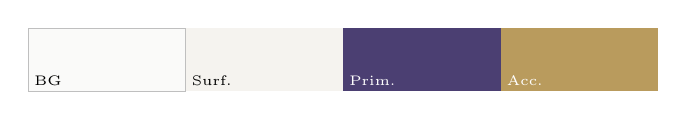
\begin{tikzpicture}
\def\w{2.0cm}\def\h{0.8cm}
\fill[swB1](0,0)rectangle(\w,\h);\draw[gray!50](0,0)rectangle(\w,\h);\node[black,anchor=south west,inner sep=2pt,font=\tiny](0,0){BG};
\fill[swB2](\w,0)rectangle(2*\w,\h);\node[black,anchor=south west,inner sep=2pt,font=\tiny] at (\w,0){Surf.};
\fill[swB3](2*\w,0)rectangle(3*\w,\h);\node[white,anchor=south west,inner sep=2pt,font=\tiny] at (2*\w,0){Prim.};
\fill[swB4](3*\w,0)rectangle(4*\w,\h);\node[white,anchor=south west,inner sep=2pt,font=\tiny] at (3*\w,0){Acc.};
\end{tikzpicture}
\par\noindent\footnotesize \#FAFAF9 $\cdot$ \#F5F3EF $\cdot$ \#4B3F72 $\cdot$ \#B99B5D $\cdot$ \#1C1A22 (text) $\cdot$ \#9A968F (muted) $\cdot$ \#E2DEDA (border)\normalsize

\subsection{Deep Blue Technology (Alternate)}
\noindent

\begin{tikzpicture}
\def\w{2.0cm}\def\h{0.8cm}
\fill[swC1](0,0)rectangle(\w,\h);\node[white,anchor=south west,inner sep=2pt,font=\tiny](0,0){BG};
\fill[swC2](\w,0)rectangle(2*\w,\h);\node[white,anchor=south west,inner sep=2pt,font=\tiny] at (\w,0){Surf.};
\fill[swC3](2*\w,0)rectangle(3*\w,\h);\node[white,anchor=south west,inner sep=2pt,font=\tiny] at (2*\w,0){Prim.};
\fill[swC4](3*\w,0)rectangle(4*\w,\h);\node[black,anchor=south west,inner sep=2pt,font=\tiny] at (3*\w,0){Acc.};
\end{tikzpicture}
\par\noindent\footnotesize \#0A0E1A $\cdot$ \#141B2E $\cdot$ \#2F5DBE $\cdot$ \#6FE3D9 $\cdot$ \#E7ECF7 (text) $\cdot$ \#7C86A3 (muted) $\cdot$ \#232B44 (border)\normalsize

\subsection{Black + One Accent (Maximum Restraint)}
\noindent

\begin{tikzpicture}
\def\w{2.0cm}\def\h{0.8cm}
\fill[swD1](0,0)rectangle(\w,\h);\node[white,anchor=south west,inner sep=2pt,font=\tiny](0,0){BG};
\fill[swD2](\w,0)rectangle(2*\w,\h);\node[white,anchor=south west,inner sep=2pt,font=\tiny] at (\w,0){Surf.};
\fill[swD3](2*\w,0)rectangle(3*\w,\h);\node[black,anchor=south west,inner sep=2pt,font=\tiny] at (2*\w,0){Prim.};
\fill[swD4](3*\w,0)rectangle(4*\w,\h);\node[white,anchor=south west,inner sep=2pt,font=\tiny] at (3*\w,0){Acc.};
\end{tikzpicture}
\par\noindent\footnotesize \#0B0B0C $\cdot$ \#151517 $\cdot$ \#EDEDED $\cdot$ \#D6472C $\cdot$ \#F4F4F4 (text) $\cdot$ \#6A6A6E (muted) $\cdot$ \#232325 (border)\normalsize

\subsection{Recommendation}
The Luxury AI Laboratory palette is recommended as the primary dark mode and Museum White as the light mode --- both share the same violet/gold accent pair, so the identity survives the toggle and directly extends an existing personal visual language across related projects. Gold (\#B99B5D) should be reserved for exactly one thing at a time on any given screen: a single CTA, a single active nav state, or a single highlighted metric.

\section{AI/ML-Specific Premium Features}

This is the section that most differentiates a research portfolio from a template, because the ``feature'' is the researcher's actual work, not a decorative effect. Table \ref{tab:aifeat_full} ranks the complete candidate feature set by genuine impact on the audiences that matter: recruiters, engineering managers, and principal investigators.

\begin{table*}[t]
\centering
\caption{Complete AI/ML Portfolio Feature Inventory and Impact Ranking}
\label{tab:aifeat_full}
\begin{tabular}{L{4.5cm}C{2.0cm}C{2.0cm}L{7.0cm}}
\toprule
\textbf{Feature} & \textbf{Recruiter impact} & \textbf{Tech-manager impact} & \textbf{Notes} \\
\midrule
Live gait-signal / embedding visualization (interactive, driven by real research data) & High & Very High & The single most valuable feature in this report --- real data, real interactivity, directly proves the claimed skill \\
Interactive model-architecture explorer (click-to-expand layers) & Med & High & Strong for technical interviewers specifically; keep a ``skip to summary'' for non-technical visitors \\
Animated research pipeline (data $\to$ preprocessing $\to$ model $\to$ evaluation, scroll-driven) & High & High & Doubles as the case-study narrative structure --- build once, reuse per project \\
Live GitHub contribution graph / activity feed & Med & Low--Med & Cheap to build (GitHub API), low risk, modest signal --- good ``proof of consistency'' widget, not a centerpiece \\
Benchmark/results dashboard (cross-validation results, transfer-learning results) & Med & Very High & What a PI or senior ML engineer actually wants to see before reading prose --- lead the case study with it \\
Live webcam pose-estimation demo & Very High (wow factor) & Med & Great portfolio centerpiece if bandwidth allows --- gate behind a clear ``try it'' button, never auto-start \\
RAG/LLM chat demo answering questions about the researcher's own work & Med & Med & Fun but risky --- a hallucinating chatbot on a portfolio undermines credibility faster than it builds it; only ship if heavily guarded/tested \\
Interactive confusion matrix / metric explorer & Low & Med & Nice-to-have depth for one flagship case study, skip elsewhere \\
3D latent-space / embedding scatter (Three.js point cloud, filterable) & Med & High & High visual payoff when it's real data (not a toy demo) --- ties directly into an existing 3D visualization codebase if one exists \\
\bottomrule
\end{tabular}
\end{table*}

We caution specifically against retrieval-augmented conversational demos answering questions about the candidate's own work: absent extensive guardrailing, a single visible hallucination in this context damages credibility more than the feature's novelty recovers.

\section{Technology Stack and Code Architecture}

\subsection{Final Recommended Stack}
\begin{table*}[t]
\centering
\caption{Complete Recommended Production Stack}
\label{tab:stack_full}
\begin{tabular}{L{2.4cm}L{3.6cm}L{9.5cm}}
\toprule
\textbf{Layer} & \textbf{Choice} & \textbf{Rationale} \\
\midrule
Framework & Next.js 15 (App Router) & Meta-frameworks are now the default professional entry point; RSC/SSR-by-default keeps JS payload low without extra effort \\
Styling & Tailwind CSS v4 + CSS variables for design tokens & Fast iteration without sacrificing a real token system; v4's native CSS engine is faster than v3's build step \\
Animation & Motion (component-level) + GSAP/ScrollTrigger (scroll timelines) + Lenis (scroll feel) & See Section VI --- both are effectively free and cover different needs cleanly \\
3D & Three.js + React Three Fiber + Drei, WebGPURenderer with WebGL fallback & Declarative, React-native, forward-compatible with WebGPU \\
Content & MDX via Contentlayer (or Velite) for case studies & Keeps long-form research writing in version control next to code --- no external CMS dependency for a personal site \\
Data visualization & D3.js (data logic) + custom SVG/Canvas rendering, or Observable Plot for quick charts & D3 for anything bespoke (embedding scatter, results plots); avoid heavy chart libraries for simple bar/line needs \\
Deployment & Vercel & Native Next.js integration, edge caching, image optimization out of the box \\
Analytics & Vercel Analytics or Plausible & Privacy-respecting, no cookie-consent friction for a portfolio \\
\bottomrule
\end{tabular}
\end{table*}

\subsection{Repository Architecture}
The recommended repository structure separates presentational components, three-dimensional scene code, shader source, animation choreography, and content into clearly bounded directories:

\begin{quote}
\ttfamily\footnotesize
src/\\
\ \ app/ \quad\# Next.js App Router routes\\
\ \ \ \ (site)/page.tsx \quad\# Home\\
\ \ \ \ (site)/work/[slug]/page.tsx\\
\ \ \ \ (site)/research/[slug]/page.tsx\\
\ \ components/\\
\ \ \ \ ui/ \quad\# Buttons, GlassSurface, MagneticLink\\
\ \ \ \ sections/ \quad\# Hero, WorkGrid, ResearchTimeline\\
\ \ three/\\
\ \ \ \ scenes/ \quad\# One file per 3D scene\\
\ \ \ \ shaders/ \quad\# .glsl / TSL node files\\
\ \ \ \ hooks/ \quad\# useResponsiveCanvas, useScrollCamera\\
\ \ animations/\\
\ \ \ \ variants.ts \quad\# Motion variant presets\\
\ \ \ \ scrollTimelines.ts \quad\# GSAP ScrollTrigger defs\\
\ \ content/\\
\ \ \ \ research/*.mdx, work/*.mdx\\
\ \ lib/ \quad\# Data fetching, GitHub API, formatting\\
\ \ styles/tokens.css \quad\# Single source of design truth\\
\ \ data/ \quad\# Static JSON: results, timeline events
\end{quote}

\subsection{Architecture Principles}
\begin{itemize}[leftmargin=*]
\item \textbf{Server/client boundary:} every 3D and heavy-animation component is a client component behind a dynamic import with \texttt{ssr:false}; everything else --- case-study text, metadata, layout --- stays a server component so it never ships JS to the client.
\item \textbf{Design tokens as the actual source of truth:} colors, spacing, and type scale live once in \texttt{tokens.css} as CSS variables, consumed by both the styling layer and any shader uniform --- never hardcode a hex value in a component.
\item \textbf{Lazy-load the heaviest contributors:} Three.js and any chart library are dynamically imported and only mount when their section scrolls into view (via \texttt{IntersectionObserver}), keeping the initial bundle lean.
\item \textbf{Never let visual code leak into content code:} MDX case-study files should be prose and data references only --- the shader that renders a visualization lives in \texttt{/three}, referenced by slug, not inlined.
\end{itemize}

\section{Performance Engineering}

Google's Core Web Vitals initiative defines three field-measured, user-centric performance thresholds, each evaluated at the 75th percentile of real Chrome User Experience Report (CrUX) traffic over a rolling 28-day window \cite{google_cwv}: Largest Contentful Paint (LCP) under 2.5\,s, Interaction to Next Paint (INP) under 200\,ms, and Cumulative Layout Shift (CLS) under 0.1. As of 2026, independent analysis of CrUX field data indicates that only approximately 43--48\% of sites pass all three thresholds simultaneously \cite{senorit_cwv, digitalapplied_cwv}, meaning that conformance is itself a differentiating signal independent of visual design quality.

\begin{table}[h]
\centering
\caption{Official Core Web Vitals Thresholds}
\label{tab:cwv_full}
\begin{tabular}{L{1.2cm}C{1.0cm}C{1.4cm}C{1.0cm}}
\toprule
\textbf{Metric} & \textbf{Good} & \textbf{Needs Impr.} & \textbf{Poor} \\
\midrule
LCP & $<$2.5s & 2.5--4.0s & $>$4.0s \\
INP & $<$200ms & 200--500ms & $>$500ms \\
CLS & $<$0.1 & 0.1--0.25 & $>$0.25 \\
\bottomrule
\end{tabular}
\end{table}

\begin{table}[h]
\centering
\caption{Portfolio-Specific Performance Budget}
\label{tab:perfbudget_full}
\begin{tabular}{L{2.6cm}L{4.4cm}}
\toprule
\textbf{Budget item} & \textbf{Target} \\
\midrule
Initial JS (excl. lazy-loaded 3D) & $<$180\,KB gzipped \\
Hero 3D asset & $<$2.5\,MB (Draco + KTX2 compressed GLB) \\
Hero image (if used instead) & $<$200\,KB, AVIF/WebP, responsive srcset \\
Font payload & $<$150\,KB total (subset glyphs, woff2, 3--4 weights max) \\
\bottomrule
\end{tabular}
\end{table}

\subsection{Specific Fixes for a 3D/Animation-Heavy Site}
\begin{itemize}[leftmargin=*]
\item \textbf{INP (the hardest metric):} break any JS task over 50\,ms; never run scene-graph rebuilds or shader recompiles on the main thread during a click/scroll response --- precompute during idle time via \texttt{requestIdleCallback}.
\item \textbf{LCP:} the hero should never be the 3D canvas itself --- render a lightweight static poster/gradient first, then progressively enhance to the WebGL scene once it's ready, so LCP is measured against something that paints instantly.
\item \textbf{CLS:} explicit width/height (or aspect-ratio) on every image, video, and canvas element; reserve layout space for any content that loads asynchronously (GitHub graph, benchmark charts).
\item \textbf{Asset compression:} Draco geometry compression plus KTX2/Basis texture compression on every GLB --- this alone typically cuts 3D asset size 80--90\%.
\item \textbf{Code-splitting discipline:} Three.js, GSAP, and any chart library are the heaviest contributors to bundle size --- dynamically import all three, gated behind viewport intersection.
\end{itemize}

\section{Accessibility and Mobile Requirements}

\subsection{Mobile Adaptation Table}
\begin{table*}[t]
\centering
\caption{Complete Desktop-to-Mobile Feature Adaptation}
\label{tab:mobile_full}
\begin{tabular}{L{4.0cm}L{12.5cm}}
\toprule
\textbf{Desktop feature} & \textbf{Mobile treatment} \\
\midrule
Custom/magnetic cursor & Removed entirely --- replace hover states with tap/press feedback \\
Full interactive 3D hero & Simplified: static poster frame or a lightweight, lower-poly scene with reduced particle count and no post-processing; never ship the desktop-resolution GLB to mobile \\
Scroll-scrubbed pinned sections & Keep, but shorten pin duration --- long pins feel worse on a phone where scroll is more physical/direct \\
Horizontal-scroll galleries & Convert to native touch-swipe with momentum (CSS scroll-snap), not a custom JS horizontal-scroll hijack \\
Glass navigation & Keep --- glass performs fine on modern mobile GPUs at nav-bar scale; just cap blur radius lower than desktop \\
\bottomrule
\end{tabular}
\end{table*}

The premium \emph{feeling} should be preserved on mobile through typography and spacing discipline more than through motion --- a beautifully set page that scrolls plainly still reads as premium; a laggy 3D scene reads as broken regardless of how good it looks on desktop.

\subsection{Complete Accessibility Requirements}
\begin{itemize}[leftmargin=*]
\item \textbf{\texttt{prefers-reduced-motion}:} every scroll-triggered and entrance animation must have a reduced/instant fallback --- this is a hard requirement, not optional polish, and both GSAP and Motion support it natively.
\item \textbf{Keyboard navigation:} every interactive 3D/canvas element needs a non-canvas fallback path (e.g., a text-based project list) reachable and operable by keyboard alone.
\item \textbf{Focus states:} visible focus rings on every interactive element --- glass/blur surfaces are especially prone to hiding focus indicators, so this must be tested specifically.
\item \textbf{Contrast:} WCAG AA minimum (4.5:1 for body text) even over glass/gradient surfaces --- requires the adaptive-tint approach from Section IV, not fixed white-on-anything.
\item \textbf{Alternative content for WebGL:} screen readers cannot parse a canvas --- every 3D scene needs an \texttt{aria-label} summary and/or an adjacent text description of what it shows.
\item \textbf{Semantic HTML underneath the visual layer:} headings, landmarks, and alt text should describe the actual content structure regardless of how it's animated on top.
\end{itemize}

A recruiter reviewing dozens of portfolios on a work laptop with reduced-motion enabled, or an engineering manager on a mid-range Android device, is a completely realistic visitor. A site that degrades gracefully for them is read --- correctly --- as more professionally engineered than one that only works in ideal conditions.

\section{Anti-Patterns: What Not to Do}

Everything catalogued below looks impressive in a screenshot or a five-second GIF and feels bad within thirty seconds of actual use --- which is exactly the window a recruiter gives a portfolio.

\subsection{Overused or Dated in 2026}
\begin{itemize}[leftmargin=*]
\item Generic mesh-gradient hero with no other identity --- now read as ``AI-generated template''
\item Glassmorphism applied to every single card on the page
\item Text-scramble/hacker decode effects on headings
\item Cursor-trail particle effects
\item Autoplaying background video with a dark overlay and centered white text (the 2018 agency-site default)
\item Parallax applied to literally everything on the page instead of one or two moments
\end{itemize}

\subsection{Bad for UX or Performance Despite Looking Good in a Demo}
\begin{itemize}[leftmargin=*]
\item Horizontal-scroll-hijacking the entire site as primary navigation
\item Long blocking intro animations with no skip option
\item Custom cursors that persist on touch devices
\item Full-resolution, uncompressed GLB/texture assets shipped to every device tier
\item Scroll-jacking that fights the user's native scroll momentum
\item A chatbot/RAG demo answering questions about the candidate that hasn't been thoroughly tested for hallucination
\end{itemize}

The tell that separates a screenshot-optimized site from a genuinely premium one: does it still feel good on the fifth interaction, on a mid-range Android phone, with reduced motion enabled, read by someone who has thirty seconds and eleven other tabs open? Every technique in this framework should survive that question before it ships.

\section{Candidate Design Directions --- Full Detail}

\subsection{Direction A --- Future Apple / Spatial Computing}
\noindent

\begin{tikzpicture}
\def\w{1.6cm}\def\h{0.7cm}
\fill[white,draw=gray!50](0,0)rectangle(\w,\h);
\fill[gray!10,draw=gray!50](\w,0)rectangle(2*\w,\h);
\fill[blue!70!white](2*\w,0)rectangle(3*\w,\h);
\fill[black](3*\w,0)rectangle(4*\w,\h);
\end{tikzpicture}
\par
\textbf{Fonts:} SF Pro-style grotesk (Inter as web-safe equivalent) throughout. \textbf{Hero:} a translucent glass card floating over a soft procedural gradient, 3D object rotating gently with cursor. \textbf{Nav:} pill-shaped floating glass bar. \textbf{Animation:} soft spring physics everywhere, minimal overshoot. \textbf{3D style:} smooth, rounded, softly lit --- visionOS-adjacent. \textbf{Cards:} translucent, heavily blurred, rounded corners. \textbf{Strengths:} instantly reads as ``premium tech,'' low execution risk. \textbf{Weaknesses:} converging with everyone else's Liquid-Glass clone in 2026 --- the least differentiated option; risks reading as derivative of Apple rather than as the candidate's own voice. \textbf{Complexity:} Medium.

\subsection{Direction B --- Luxury AI Laboratory (Recommended)}
\noindent

\begin{tikzpicture}
\def\w{1.6cm}\def\h{0.7cm}
\fill[swA1](0,0)rectangle(\w,\h);
\fill[swA2](\w,0)rectangle(2*\w,\h);
\fill[swA4](2*\w,0)rectangle(3*\w,\h);
\fill[swA2!50!white](3*\w,0)rectangle(4*\w,\h);
\end{tikzpicture}
\par
\textbf{Fonts:} Fraunces display + Inter body + JetBrains Mono for data. \textbf{Hero:} near-black background, restrained gold accent, oversized editorial headline, one real 3D research artifact (e.g., a gait-signal point cloud or skeleton rig) rendered with quiet precision --- no particle spectacle. \textbf{Nav:} minimal glass bar, text-only links, no icons. \textbf{Animation:} scroll-driven editorial reveals, GSAP-choreographed case-study walkthroughs. \textbf{3D style:} scientific, precise, monochrome-lit --- think architectural render, not game engine. \textbf{Cards:} flat, hairline-bordered, generous whitespace. \textbf{Case studies:} led by a quantitative result, followed by a scroll-driven pipeline diagram, followed by an honest methods/limitations section. \textbf{Strengths:} directly extends an existing Museum-White-style visual language; content-forward, which plays to a research candidate's actual strength (real research); reads as ``researcher,'' not ``agency.'' \textbf{Weaknesses:} lower wow-factor-in-a-screenshot than Direction C; requires genuinely strong writing to carry it, since there is nowhere to hide behind spectacle. \textbf{Complexity:} Medium.

\subsection{Direction C --- Experimental AI / Creative Technology}
\noindent

\begin{tikzpicture}
\def\w{1.6cm}\def\h{0.7cm}
\fill[swC1](0,0)rectangle(\w,\h);
\fill[swC2](\w,0)rectangle(2*\w,\h);
\fill[violet](2*\w,0)rectangle(3*\w,\h);
\fill[violet!20!white](3*\w,0)rectangle(4*\w,\h);
\end{tikzpicture}
\par
\textbf{Fonts:} Space Grotesk display, kinetic/animated headline treatment. \textbf{Hero:} full-viewport WebGPU particle/shader scene, cursor-reactive, unconventional radial or spatial navigation. \textbf{Animation:} generative, shader-driven, camera moves through a 3D environment between sections. \textbf{3D style:} maximal, compute-shader particle fields, procedural geometry. \textbf{Strengths:} highest raw wow-factor, most likely to win an actual Awwwards nomination. \textbf{Weaknesses:} highest build/maintenance cost by a wide margin; risks burying the candidate's actual research content under spectacle --- the wrong trade for a recruiter audience who has 30--90 seconds; hardest to keep performant across device tiers. \textbf{Complexity:} Very High.

\subsection{Recommendation}
Direction B is recommended as the primary system, augmented with exactly two contained instances of Direction C's techniques: a real-time particle/shader hero moment built from the candidate's actual research data (not decorative noise), and one scroll-driven camera sequence through a research-pipeline visualization. This captures Awwwards-adjacent spectacle at the two moments of highest attention without diluting the editorial credibility that Direction B protects everywhere else, and matches the empirical pattern from Section II: 2026's highest-scoring Developer Award recipients pick one or two techniques and execute them at a level almost nobody else attempts, rather than distributing effort across many.

\section{Final Blueprint --- The Complete Recommended Build}

\textbf{Overall creative concept:} ``A researcher's laboratory, rendered with the same visual intelligence Apple applies to a product page.'' Restrained luxury-editorial base (Direction B) with two precision-built real-data 3D moments. Every visual choice should be traceable to a real fact about the candidate's work --- never decoration for its own sake.

\textbf{Visual language and palette:} Luxury AI Laboratory dark palette as primary; Museum White as an explicit light-mode toggle (both share the violet/gold accent pair; see Section VIII).

\textbf{Typography:} Fraunces for the wordmark and section headlines only; Inter for all body/UI text; JetBrains Mono for every metric, benchmark number, and code reference.

\textbf{Navigation:} Fixed glass pill bar, text-only links (Work $\cdot$ Research $\cdot$ About $\cdot$ Contact), morphing to a compact state on scroll via Motion's layout animation.

\textbf{Hero:} Full-bleed near-black section. Oversized Fraunces headline with word-by-word GSAP reveal. Beneath the fold-line, a real-time R3F point-cloud/skeleton visualization sourced from actual research data, GPU-instanced, subtly cursor-reactive. Static poster frame loads first for LCP; canvas hydrates after.

\textbf{3D system:} Three.js + R3F + Drei, WebGPURenderer with WebGL fallback. Two flagship 3D moments only (hero plus one case-study camera sequence); Draco/KTX2-compressed GLB throughout.

\textbf{Animation system:} Motion for component-level interaction; GSAP + ScrollTrigger for the hero reveal and case-study scroll narratives; Lenis underneath for scroll feel.

\textbf{Sections:} Hero $\to$ Selected Research (flagship case studies) $\to$ Selected Work (internships, side projects, other builds) $\to$ Technical Stack (bento grid) $\to$ About $\to$ Contact. A generic ``Skills'' wall of badges should be skipped --- competency should be folded into the case studies themselves.

\textbf{Case studies:} Structured like a scientific publication crossed with a product launch: hero metric first, then a scroll-driven pipeline diagram, then an honest methods/limitations section --- null-result and power-analysis content belongs here as a credibility asset, not something to hide.

\textbf{Footer, mobile, accessibility, performance:} Minimal footer (contact, resume download, GitHub/LinkedIn, last-updated date). Mobile drops the custom cursor and simplifies the hero to a lower-poly/static variant per Section XII. Full \texttt{prefers-reduced-motion} compliance and keyboard-operable fallbacks for every 3D element per Section XII. Performance budget enforced per Section XI: LCP $<$2.5\,s, INP $<$200\,ms, CLS $<$0.1, initial JS $<$180\,KB.

\textbf{Technology stack and deployment (restated):} Next.js 15 App Router $\cdot$ Tailwind v4 $\cdot$ Motion + GSAP/ScrollTrigger + Lenis $\cdot$ Three.js/R3F/Drei with WebGPURenderer $\cdot$ MDX via Contentlayer for case-study content $\cdot$ D3 for bespoke data visualization $\cdot$ deployed on Vercel with Vercel Analytics.

\section{Complete Feature Prioritization Matrix}

Table \ref{tab:priomatrix_full} reproduces the complete 24-item prioritization matrix in full, with no items omitted, classified into four tiers: S (absolutely worth doing), A (high-value premium), B (nice-to-have), and C (gimmick --- skip).

\begin{table*}[t]
\centering
\caption{Complete Feature Prioritization Matrix (24 Items)}
\label{tab:priomatrix_full}
\begin{tabular}{L{5.0cm}C{1.2cm}C{1.4cm}C{1.6cm}C{1.6cm}C{1.0cm}}
\toprule
\textbf{Feature} & \textbf{Wow} & \textbf{UX Value} & \textbf{Difficulty} & \textbf{Perf. Cost} & \textbf{Tier} \\
\midrule
Real-data 3D hero (e.g., gait point cloud) & 9 & 8 & High & Med & S \\
Editorial word-by-word text reveal & 6 & 7 & Low & Low & S \\
Magnetic buttons / spring underlines & 5 & 8 & Low & Low & S \\
Case-study scroll-pinned pipeline diagram & 8 & 8 & Med & Med & S \\
Benchmark/results dashboard & 6 & 9 & Med & Low & S \\
Glass navigation bar & 6 & 7 & Med & Low & S \\
Variable-font weight hover animation & 5 & 6 & Low & Low & S \\
3D card tilt on hover & 6 & 6 & Low & Low & A \\
Custom contextual cursor (desktop only) & 7 & 5 & Med & Low & A \\
Live GitHub activity graph & 4 & 5 & Low & Low & A \\
3D embedding/latent-space scatter (real data) & 8 & 7 & High & Med & A \\
Interactive model-architecture explorer & 7 & 7 & High & Med & A \\
Ambient GPU particle background & 6 & 4 & Med & Med & B \\
Dark/light mode toggle & 3 & 6 & Low & Low & B \\
Cursor-following spotlight (dark sections) & 5 & 4 & Low & Low & B \\
Live webcam pose-estimation demo & 9 & 5 & High & High & B \\
RAG/LLM chatbot about own work & 6 & 3 & High & Med & B \\
3D typography / extruded wordmark & 6 & 3 & Med & Low & B \\
Full navigable 3D world / driveable scene & 9 & 2 & Very High & High & C \\
Text-scramble/decode hover effect & 4 & 2 & Low & Low & C \\
Cursor particle trails & 4 & 2 & Low & Low & C \\
Elastic/liquid button morph & 5 & 2 & Med & Low & C \\
Horizontal-scroll-hijacked full site & 6 & 2 & High & Med & C \\
Full-page shader background everywhere & 6 & 2 & Med & High & C \\
\bottomrule
\end{tabular}
\end{table*}

\section{Complete Launch-Readiness Checklist}

This section reproduces the full, unabridged launch checklist across all eight categories, with every item preserved.

\subsection{Design and Brand}
\begin{itemize}[leftmargin=*]
\item Single coherent direction chosen (Section XIV) --- no mixing of unrelated visual languages
\item Design tokens (color/type/spacing) defined once, consumed everywhere
\item Consistent easing curve and duration scale across every animation
\item Palette restricted to one or two hues across six to eight stepped values
\end{itemize}

\subsection{Typography}
\begin{itemize}[leftmargin=*]
\item Type scale defined and used exactly (no ad hoc sizes)
\item Negative tracking applied above 40\,px display sizes
\item Fonts subsetted, woff2, four weights or fewer loaded
\end{itemize}

\subsection{Content}
\begin{itemize}[leftmargin=*]
\item Real metrics lead every case study, not buried in prose
\item Limitations/null-results honestly presented (credibility asset)
\item Resume/CV downloadable, kept current
\end{itemize}

\subsection{3D and Animation}
\begin{itemize}[leftmargin=*]
\item GLB assets Draco + KTX2 compressed
\item Static poster frame precedes canvas hydration
\item Frame budget holds 60\,fps during scroll on a mid-tier laptop
\item Every animation has a \texttt{prefers-reduced-motion} fallback
\end{itemize}

\subsection{Performance}
\begin{itemize}[leftmargin=*]
\item LCP $<$2.5\,s, INP $<$200\,ms, CLS $<$0.1 at p75 (real-device testing, not just Lighthouse)
\item Initial JS bundle $<$180\,KB gzipped
\item Three.js/GSAP/charts lazy-loaded behind intersection observers
\item Images AVIF/WebP with explicit dimensions
\end{itemize}

\subsection{Accessibility}
\begin{itemize}[leftmargin=*]
\item WCAG AA contrast, including over glass/gradient surfaces
\item Full keyboard operability, visible focus states
\item Text alternative for every canvas/WebGL scene
\item Custom cursor fully removed on touch devices
\end{itemize}

\subsection{Mobile}
\begin{itemize}[leftmargin=*]
\item 3D scenes simplified/lower-poly on mobile, not just scaled down
\item Touch-native swipe (scroll-snap) instead of hijacked horizontal scroll
\item Tested on an actual mid-range Android device, not just desktop devtools emulation
\end{itemize}

\subsection{SEO, Technical, Code Quality, and Deployment}
\begin{itemize}[leftmargin=*]
\item Semantic HTML/landmarks under every visual layer
\item Open Graph/meta tags for every case study
\item Sitemap and robots.txt configured
\item Server/client component boundaries deliberate, not accidental
\item Shaders/3D isolated from application component logic
\item Continuous-integration pipeline runs Lighthouse/Core-Web-Vitals checks on every deploy
\item Analytics configured (privacy-respecting)
\end{itemize}

\section{Conclusion}

This paper has presented a complete, unabridged framework for designing a premium personal research portfolio, synthesizing 2026 award-circuit practice, current browser platform capability, and Core Web Vitals performance constraints, without compressing any table, ranking, or checklist item from the underlying research for length. The central empirical claim --- that perceived production value correlates with technique restraint and content fidelity rather than technique density --- is supported by comparative analysis of current Developer Award recipients and by the structural logic of the target audience's evaluation process. For a research-track candidate specifically, the highest-leverage design decision available is the use of one's own experimental data as the primary visual and interactive asset, which is simultaneously the most differentiated content achievable and direct evidence of the technical capability under evaluation. The complete specification in Sections X--XVII is intended to be directly implementable without further research: stack, architecture, budget, accessibility requirements, prioritization, and checklist are all reproduced in full above.

\begin{thebibliography}{00}

\bibitem{talent500_2026} Talent500 Engineering Blog, ``8 Web Development Trends for 2026: AI, Edge, TypeScript,'' 2026. [Online]. Available: https://talent500.com/blog/web-development-trends-2026-2/

\bibitem{dsf_2026} Digital Strategy Force, ``Why Are Immersive Experiences Dominating the 2026 Awwwards?,'' 2026. [Online]. Available: https://digitalstrategyforce.com/journal/why-are-immersive-experiences-dominating-the-2026-awwwards/

\bibitem{awwwards_sotm} Awwwards, ``Sites of the Month,'' 2026. [Online]. Available: https://www.awwwards.com/websites/sites\_of\_the\_month/

\bibitem{hontran_2026} H. Tran, ``10 Award-Winning Websites of 2026, Judged,'' 2026. [Online]. Available: https://www.hontran.dev/blog/best-award-winning-websites-2026

\bibitem{figma_2026} Figma Resource Library, ``12 Defining Web Development Trends for 2026,'' 2026. [Online]. Available: https://www.figma.com/resource-library/web-development-trends/

\bibitem{logrocket_trends2026} LogRocket Blog, ``The 8 Trends That Will Define Web Development in 2026,'' 2026. [Online]. Available: https://blog.logrocket.com/8-trends-web-dev-2026/

\bibitem{openreplay_2026} OpenReplay Blog, ``Motion vs GSAP: Do You Need Both?,'' 2026. [Online]. Available: https://blog.openreplay.com/motion-vs-gsap/

\bibitem{smashingapps_2026} SmashingApps, ``The Complete Guide to Best Free JavaScript Animation Libraries in 2026,'' 2026. [Online]. Available: https://www.smashingapps.com/best-free-javascript-animation-libraries-in-2026/

\bibitem{hontran_gsap2026} H. Tran, ``GSAP vs Framer Motion in 2026: An Honest Verdict,'' 2026. [Online]. Available: https://www.hontran.dev/blog/gsap-vs-framer-motion

\bibitem{motion_docs} Motion, ``GSAP vs Motion: A Detailed Comparison,'' 2026. [Online]. Available: https://motion.dev/docs/gsap-vs-motion

\bibitem{apple_liquidglass} Apple Inc., ``Apple Introduces a Delightful and Elegant New Software Design,'' Apple Newsroom, 2025. [Online]. Available: https://www.apple.com/newsroom/2025/06/apple-introduces-a-delightful-and-elegant-new-software-design/

\bibitem{css_tricks_glass} CSS-Tricks, ``Getting Clarity on Apple's Liquid Glass,'' 2026. [Online]. Available: https://css-tricks.com/getting-clarity-on-apples-liquid-glass/

\bibitem{logrocket_glass} LogRocket Blog, ``Adopting Apple's Liquid Glass: Examples and Best Practices,'' 2025. [Online]. Available: https://blog.logrocket.com/ux-design/adopting-liquid-glass-examples-best-practices/

\bibitem{ekino_glass} ekino-france, ``Liquid Glass in CSS (and SVG),'' Medium, 2025. [Online]. Available: https://medium.com/ekino-france/liquid-glass-in-css-and-svg-839985fcb88d

\bibitem{logrocket_svgglass} LogRocket Blog, ``How to Create Liquid Glass Effects with CSS and SVG,'' 2026. [Online]. Available: https://blog.logrocket.com/how-create-liquid-glass-effects-css-and-svg/

\bibitem{threejs_resources} Three.js Resources, ``GSAP --- Animation for Three.js,'' 2026. [Online]. Available: https://threejsresources.com/tool/gsap

\bibitem{webgpu_showcase} WebGPU.com, ``React Three Fiber Community Showcase,'' 2026. [Online]. Available: https://www.webgpu.com/tag/react-three-fiber/

\bibitem{google_cwv} Google Search Central, ``Understanding Core Web Vitals and Google Search Results,'' 2025. [Online]. Available: https://developers.google.com/search/docs/appearance/core-web-vitals

\bibitem{senorit_cwv} Senorit, ``Core Web Vitals 2026: LCP, INP \& CLS Thresholds,'' 2026. [Online]. Available: https://senorit.de/en/blog/core-web-vitals-2026

\bibitem{digitalapplied_cwv} Digital Applied, ``Core Web Vitals 2026: INP, LCP \& CLS Optimization,'' 2026. [Online]. Available: https://www.digitalapplied.com/blog/core-web-vitals-2026-inp-lcp-cls-optimization-guide

\end{thebibliography}

\end{document}
